
\documentclass[12pt,hyperref={CJKbookmarks=true}]{beamer} %14pt为字体尺寸,默认值11pt.有8-12;14;17;20;bigger;smaller
\usepackage{ifthen}
%\usepackage[a3paper,landscape,showframe,margin=1.25in]{geometry}
%\usepackage[a3paper,landscape,margin=1.1in]{geometry}
\usepackage[a3paper,landscape,top=1.25in,bottom=0.8in,left=1in,right=1in]{geometry}
\usepackage{tikz,units}
\usepackage{circuitikz}
\usepackage{subfig}
\usetikzlibrary{backgrounds,circuits.ee.IEC.relay}
\usetikzlibrary{positioning}
\usepackage{tikzsymbols}
\usepackage{pgffor}
\usetikzlibrary {math}
\usepackage{lastpage}
\usepackage{fancyhdr}
\pagestyle{fancy}
\fancyhf{}
\fancyhead[ER,OL]{\heiti \zihao{-5} 热工专业图纸}
\fancyhead[OR,EL]{\heiti \zihao{-5} \leftmark}
\fancyfoot[CE,CO]{热工专业图纸~第~\thepage~页(共 \pageref{LastPage} 页)}
\renewcommand{\headrulewidth}{0.4pt}
\renewcommand{\footrulewidth}{0.4pt}
\tikzset{
box/.style={rectangle,minimum height=17pt,minimum width=20pt,text=red}
}
\tikzset{
boxA/.style={rectangle,minimum height=17pt,minimum width=20pt,draw=black}
}
\tikzset{
boxB/.style={rectangle,minimum height=17pt,minimum width=30pt,draw=black}
}
\tikzset{
boxC/.style={rectangle,minimum height=17pt,minimum width=120pt,draw=black}
}
\tikzset{
boxD/.style={minimum width=140pt,above left}
}
 % 載入封包與文檔配置
\usepackage{verbatim}
%\usepackage{multicol}分栏
\usepackage{tikz}
\usetikzlibrary{backgrounds,circuits.ee.IEC.relay}
%\usepackage[autoplay,loop]{animate}
\usepackage{animate}
\tikzset{
dpu/.style={rectangle,rounded corners=2pt,
minimum width=35pt,minimum height=40pt,inner sep=5pt,
draw=black,fill=black!20,scale=0.8},
switch/.style={rectangle,rounded corners=5pt,
minimum width=15pt,minimum height=50pt,inner sep=5pt,
draw=black,fill=black!20}
}
\tikzset{
box/.style = {rectangle,draw=black,fill=lightgray}
}



\makeatletter
\def\progressbar@progressbar{} % the progress bar
\newcount\progressbar@tmpcounta% auxiliary counter
\newcount\progressbar@tmpcountb% auxiliary counter
\newdimen\progressbar@pbht %progressbar height
\newdimen\progressbar@pbwd %progressbar width
\newdimen\progressbar@rcircle % radius for the circle
\newdimen\progressbar@tmpdim % auxiliary dimension

\progressbar@pbwd=\linewidth
\progressbar@pbht=1pt
\progressbar@rcircle=2.5pt

% the progress bar
\def\progressbar@progressbar{%

    \progressbar@tmpcounta=\insertframenumber
    \progressbar@tmpcountb=\inserttotalframenumber
    \progressbar@tmpdim=\progressbar@pbwd
    \multiply\progressbar@tmpdim by \progressbar@tmpcounta
    \divide\progressbar@tmpdim by \progressbar@tmpcountb

  \begin{tikzpicture}
    \draw[pbblue!30,line width=\progressbar@pbht]
      (0pt, 0pt) -- ++ (\progressbar@pbwd,0pt);

    \filldraw[pbblue!30] %
      (\the\dimexpr\progressbar@tmpdim-\progressbar@rcircle\relax, .5\progressbar@pbht) circle (\progressbar@rcircle);

    \node[draw=pbblue!30,text width=4em,align=center,inner sep=1pt,
      text=pbblue!70,anchor=east] at (0,0) {\textnormal{%
             \pgfmathparse{\insertframenumber*100/\inserttotalframenumber}%
             \pgfmathprintnumber[fixed,precision=2]{\pgfmathresult}\,\%%
        }%
};
  \end{tikzpicture}%
}

\addtobeamertemplate{headline}{}
{%
  \begin{beamercolorbox}[wd=\paperwidth,ht=4ex,center,dp=1ex]{white}%
    \progressbar@progressbar%
  \end{beamercolorbox}%
}
\makeatother








\begin{document}
	
	\kaishu
	
	\title{给煤机原理及维护培训}
\subtitle{VEG20650}
	\author{热控专业}
	\institute[检修部热控班组]{热控班组}
	\date{\today}
	\begin{frame}
		\titlepage
	\end{frame}
\begin{frame}{\textbf{目录}}
\begin{multicols}{2}
\tableofcontents
\end{multicols}
\end{frame}
	\section{给煤机控制系统}
	
\begin{frame}{给煤机工作原理}{控制原理示意图}
\begin{tikzpicture}
\node[box] (Qt) at(5,4) {控制仪表};
\node[box] (HZ) at(0,0) {变频器};
\node[box] (Vt) at(10,0) {转速探头};
\node[box] (SP) at(0,4) {设定流量};
\node[box] (qt) at(10,4) {称重传感器};
\draw[->] (SP) -- node[above]{4-20mA}(Qt);
\draw[<-] (Qt) -- node[above]{qt:瞬时负荷}(qt);
\draw[<-] (Qt) -- node[above,sloped]{Vt:瞬时速度}(Vt);
\draw[->] (Qt) -- node[above,sloped]{4-20mA}(HZ);
\draw[->] (HZ) -- node[above]{电机}(Vt);
\end{tikzpicture}	
	\end{frame}
\subsection{给煤机控制回路组成部件}
\begin{frame}{给煤机工作原理}{给煤机控制回路组成部件}
\begin{block}{系统组成部件及作用}
\begin{description}
				\item[控制仪表]核心设备,负责接收远方指令、采集信号,运算调节仪表型号:VEG 20650/VWF 20650
				\item[称重传感器]成对安装,安装在称重托辊两侧,测量皮带称量段上的瞬时负荷qt
				\item[磁电转速探头]安装在电机尾部风扇罩上,检测皮带电机尾部齿轮盘脉冲信号
				\item[变频器]接收控制仪表输出的AO控制信号,控制皮带电机转速
				\item[控制回路]给煤机动力回路、控制回路
				
			\end{description}
		\end{block}

	\end{frame}
\subsection{工作原理概述}
\begin{frame}{给煤机工作原理}{工作原理概述}
\begin{exampleblock}{工作原理}
正常工作状态下,物料随皮带被拖出布于皮带的工作面上,此时称量段上瞬时平均物料重力通过称量机构成线性关系作用在称重传感器上。传感器所受的重力Pt为:Pt=CqtL(Kg)\\
\text{皮带称量段上的瞬时负荷}qt:Kg/m \text{有效称量段长度}L:m \text{比例系数}C\\
根据惠更斯桥路原理的电阻应变传感器,其电信号输出与所受重力大小成正比。因此,称重传感器输出的电信号就是皮带瞬时负荷的代表量\\
\text{瞬时给料量} Qt=qtVt(Kg/s) \text{皮带瞬时速度}Vt:m/s
瞬时给料量作为测量值输入运算控制器,与设定值进行比较,预算控制器即可根据偏差大小和方向,输出相应调节信号来改变皮带速度,使给料量趋向最终达到设定的目标值
		\end{exampleblock}
	\end{frame}
\subsection{控制仪表接线}

\begin{frame}{给煤机工作原理}{控制仪表接线及信号类型}
\begin{block}{控制仪表接线及信号类型}
				\begin{description}
\item[电源:]  X2-1、X2-2 来至DCS机柜内24VDC电源(带保险)
				\item[给煤量指令:]  X8-1、X8-2 来至DCS AO卡件4-20mA信号
				\item[称重传感器A:]  X10-3、X10-4、X10-5
				\item[称重传感器B:]  X10-6、X10-7、X10-8
				\item[皮带  转速]  X10-1、X10-2 来至转速探头的脉冲信号
\item[至变频器信号:]  X8-4、X8-5 输出至变频器控制信号
\item[给煤量反馈:]  X12-8、X12-9 输出至DCS AI卡件4-20mA信号
\item[累计给煤量:]  X1-5、X1-6 输出至DCS DPI卡件脉冲信号
			\end{description}

		\end{block}

	\end{frame}
\subsection{控制仪表操作与显示}
	
	\begin{frame}{给煤机电气原理}{控制仪表操作与显示}
		\begin{block}{控制仪表显示}
				\begin{description}
				\item[顶部显示区:]  运行状态(左上角转动十字)和工作模式
				\item[故障显示区:]  显示事件代码和简单的描述
				\item[上部显示区:]  实际测量数据
				\item[下部显示区:]  可自定义的实际数据显示
			\end{description}

		\end{block}
\begin{block}{控制仪表操作}
				\begin{description}
				\item[启动按钮:]  启动计量
				\item[停止按钮:]  停止计量
				\item[删除按钮:]  清除事件和故障复位
			\end{description}

		\end{block}
	\end{frame}
\begin{frame}{给煤机电气原理}{控制仪表控制模式}
		\begin{block}{称重控制模式(闭环控制)}
				根据流量反馈值和设定值的偏差总是输出调节信号,使反馈值跟踪流量设置值
			

		\end{block}
\begin{exampleblock}{容积控制模式(开环控制)}
			在容积控制模式下,皮带驱动电机的转速与流量给定值成正比例。皮带负荷不再参与控制\\
标定程序、零点设定程序、去皮程序、量程标定程序以及皮带整圈脉冲数设定程序都必须在容积控制模式下操作
		\end{exampleblock}
\begin{alertblock}{正常生产控制方式:称重控制模式!!!}
			在显顶部显示区有V容积控制模式,没有V表示称重控制模式
		\end{alertblock}
	\end{frame}
\section{给煤机标定功能}
	\begin{frame}{给煤机标定功能}{标定功能}
		
\begin{block}{标定功能}
				\begin{description}
				\item[皮带整圈脉冲数设定:]  得到皮带运行整圈转速探头测得脉冲数
\item[去皮程序:]在试运行、维修、维护期间,获取基本皮重
\item[调零程序:]获取正常运行中的零点偏差
\item[量程标定程序:]对秤计量准确性进行检查
			

				\end{description}
\end{block}
	\begin{block}{标定注意事项}
\begin{enumerate}
\item  皮带运行中无跑偏或剐蹭
				\item  所有标定必须在容积模式进行
				\item  所有标定程序采用密码进行保护,密码7353
				\item  程序运行时,不进行累加,模拟输出置于最低值
				\end{enumerate}
				
\end{block}
	\end{frame}
\section{ETS系统}
\subsection{ETS控制系统参数、组成}
\begin{frame}{ETS控制系统}{系统参数、组成}
  		\begin{block}{控制器参数(CPU 226 CN AC/DC/RLY)}
  		\begin{enumerate}
				\item 220VAC电源/DI为24VDC/输出为继电器输出
				\item  输出并联实现控制器冗余
%\item   仪表工作在容积控制模式	
			\end{enumerate}
\end{block}
\begin{exampleblock}{冗余输出方式}
  		\begin{enumerate}
				\item 通道输出并联控制继电器线圈
				\item  皮带必须处于恒数运行状态
%\item   仪表工作在容积控制模式	
			\end{enumerate}
\end{exampleblock}
\begin{alertblock}{与上位机交互方式}
  		通过通讯模块与DEH系统上位机实现交互
\end{alertblock}
	\end{frame}
\subsection{关闭主汽门}
	\begin{frame}{ETS控制系统输出}{关闭主汽门}
  		\begin{columns}
			\column{.5\textwidth}
\begin{figure}
%\centering
\includegraphics[angle=90,width=150pt,trim=550 200 40 100,clip]{picture/ets8.pdf}\\
\includegraphics[angle=0,width=150pt,trim=0 350 50 100,clip]{picture/plc8.pdf}
%\caption{两线制接线图}
	
\end{figure}
	\column{.5\textwidth}
\begin{block}{磁力断路油门}
			\begin{enumerate}
				\item  工作电压220VAC
				\item  主汽门供油
				\end{enumerate}
\end{block}
\begin{exampleblock}{控制回路}
			\begin{enumerate}
				\item PLC输出与手动停机
				\item J101和J102继电器并联
				\end{enumerate}
\end{exampleblock}
\begin{alertblock}{控制系统}
				\begin{enumerate}
				\item Q0.0和Q0.1并联
				\item 动作时间15S
				\end{enumerate}
\end{alertblock}
		\end{columns}
	\end{frame}
\subsection{关闭抽汽逆止阀}
\begin{frame}{ETS控制系统输出}{关闭抽汽逆止阀}
  		\begin{columns}
			\column{.5\textwidth}
\begin{figure}
%\centering
\includegraphics[angle=90,width=150pt,trim=250 400 420 100,clip]{picture/ets8.pdf}\\
\includegraphics[angle=0,width=150pt,trim=0 350 50 250,clip]{picture/plc9.pdf}\\
\includegraphics[angle=0,width=150pt,trim=0 550 50 50,clip]{picture/plc10.pdf}
%\caption{两线制接线图}
	
\end{figure}
	\column{.5\textwidth}
\begin{block}{抽汽逆止阀}
			\begin{enumerate}
				\item  工作电压220VAC
				\item  失电状态?
				\end{enumerate}
\end{block}
\begin{exampleblock}{控制回路}
			\begin{enumerate}
				\item 手动开、关
				\item ETS柜按钮操作
				\end{enumerate}
\end{exampleblock}
\begin{alertblock}{控制系统}
				\begin{enumerate}
				\item 软按钮开、关
				\item DEH系统通讯操作
				\end{enumerate}
\end{alertblock}
		\end{columns}
	\end{frame}
\subsection{关联其他系统}
\begin{frame}{ETS控制系统输出}{关联其他系统}
  		\begin{columns}
			\column{.5\textwidth}
\begin{figure}
%\centering
\includegraphics[angle=90,width=150pt,trim=400 400 170 100,clip]{picture/ets8.pdf}\\
\includegraphics[angle=0,width=150pt,trim=0 150 50 300,clip]{picture/plc8.pdf}
%\caption{两线制接线图}
	
\end{figure}
	\column{.5\textwidth}
\begin{block}{至电气}
			机跳电保护
\end{block}
\begin{exampleblock}{DCS系统}
			显示ETS停机信号
\end{exampleblock}
\begin{alertblock}{DEH系统}
				\begin{enumerate}
				\item SOE
				\end{enumerate}
\end{alertblock}
		\end{columns}
	\end{frame}
\subsection{}
\begin{frame}{ETS控制系统输入}{超速保护举例}
  		\begin{columns}
			\column{.5\textwidth}
\begin{figure}
%\centering
\includegraphics[angle=90,width=50pt,trim=550 800 40 100,clip]{picture/ets4.pdf}
\includegraphics[angle=90,width=50pt,trim=530 900 50 100,clip]{picture/ets5.pdf}
\\
\includegraphics[angle=0,width=150pt,trim=0 600 0 100,clip]{picture/plc2.pdf}\\
\includegraphics[angle=0,width=150pt,trim=0 600 0 100,clip]{picture/plc5.pdf}\\
\includegraphics[angle=0,width=150pt,trim=50 930 0 80,clip]{picture/ets9.pdf}
%\caption{两线制接线图}
	
\end{figure}
	\column{.5\textwidth}
\begin{block}{磁力断路油门}
			\begin{enumerate}
				\item  工作电压220VAC
				\item  主汽门供油
				\end{enumerate}
\end{block}
\begin{exampleblock}{控制回路}
			\begin{enumerate}
				\item PLC输出与手动停机
				\item J101和J102继电器并联
				\end{enumerate}
\end{exampleblock}
\begin{alertblock}{控制系统}
				\begin{enumerate}
				\item Q0.0和Q0.1并联
				\item 动作时间15S
				\end{enumerate}
\end{alertblock}
		\end{columns}
	\end{frame}
\subsection{实现与上位机交互}
\begin{frame}{ETS控制系统输出}{实现与上位机交互}
  		\begin{columns}
			\column{.5\textwidth}
\begin{figure}
%\centering
\includegraphics[angle=0,width=70pt,trim=0 0 0 0,clip]{picture/i.png}
\includegraphics[angle=0,width=70pt,trim=0 0 0 0,clip]{picture/q.png}\\
\includegraphics[angle=0,width=70pt,trim=0 50 50 50,clip]{picture/plc12.pdf}
\includegraphics[angle=0,width=70pt,trim=0 50 50 50,clip]{picture/plc13.pdf}
%\caption{两线制接线图}
	
\end{figure}
	\column{.5\textwidth}
\begin{block}{PROFIBUS通讯}
			\begin{enumerate}
				\item  工作电压220VAC
				\item  主汽门供油
				\end{enumerate}
\end{block}
\begin{exampleblock}{PLC数据打包}
			\begin{enumerate}
				\item PLC输出与手动停机
				\item J101和J102继电器并联
				\end{enumerate}
\end{exampleblock}
\begin{alertblock}{DEH系统数据解包}
				\begin{enumerate}
				\item Q0.0和Q0.1并联
				\item 动作时间15S
				\end{enumerate}
\end{alertblock}
		\end{columns}
	\end{frame}
\section{DCS系统请求停机}
\subsection{DCS请求停机保护}
\begin{frame}{DCS请求停机保护}{保护内容及触发方式}
  		\begin{block}{保护内容}
  		\begin{enumerate}
				\item 汽轮机支撑轴承金属温度高且回油温度高
				\item 汽轮机后轴承金属温度高且回油温度高
				\item 发电机前轴承金属温度高且回油温度高
				\item 发电机后轴承金属温度高且回油温度高
				\item 汽轮机轴振动高
				\item 汽轮机油箱油位报警
%\item   仪表工作在容积控制模式	
			\end{enumerate}
\end{block}
\begin{alertblock}{保护触发方式}
  		\begin{enumerate}
			\item DCS发出三个请求停机信号至ETS系统
			\item ETS系统内三取二判断后触发DCS请求停机保护	
			\end{enumerate}
\end{alertblock}
	\end{frame}
\subsection{DCS请求停机保护}
\begin{frame}{DCS请求停机保护}{保护内容及触发方式}
  		\begin{block}{保护内容}
  		\begin{enumerate}
				\item 汽轮机支撑轴承金属温度高且回油温度高
				\item 汽轮机后轴承金属温度高且回油温度高
				\item 发电机前轴承金属温度高且回油温度高
				\item 发电机后轴承金属温度高且回油温度高
				\item 汽轮机轴振动高
				\item 汽轮机油箱油位报警
%\item   仪表工作在容积控制模式	
			\end{enumerate}
\end{block}
\begin{alertblock}{保护触发方式}
  		\begin{enumerate}
			\item DCS发出三个请求停机信号至ETS系统
			\item ETS系统内三取二判断后触发DCS请求停机保护	
			\end{enumerate}
\end{alertblock}
	\end{frame}
\subsection{去皮程序}
\begin{frame}{给煤机标定功能}{去皮程序:TW}
  		\begin{block}{标定程序作用}
  		记录皮带运行一整圈或几个整圈的零点平均误差并在以后得操作中消除此误差。
\end{block}
\begin{exampleblock}{标定程序执行的前提条件}
  		\begin{enumerate}
				\item 皮带必须处于空载状态
				\item  对处于称量区域内的秤体机械设备进行清扫
				\item   秤必须以容积方式运行,键盘控制,设定值为额定流量值			
			\end{enumerate}
\end{exampleblock}
\begin{alertblock}{标定程序结束后影响}
  		按下确认键后自动更改参数P04.04(基本皮重),参数P04.05(皮重修正值)被置零
\end{alertblock}
	\end{frame}
\begin{frame}{给煤机标定功能}{皮带整圈脉冲数设定:LB参数}
  		\begin{columns}
			\column{.5\textwidth}
\begin{figure}
%\centering
%\includegraphics[angle=0,width=150pt,trim=0 0 0 0,clip]{picture/TWing.jpg}\\
%\includegraphics[angle=0,width=150pt,trim=0 0 0 0,clip]{picture/TWed.jpg}
%\caption{两线制接线图}
	
\end{figure}
	\column{.5\textwidth}
\begin{block}{回路特点}
			\begin{enumerate}
				\item  与预先去皮比较的皮重偏差
				\item  总皮重值相对于额定负荷
				\end{enumerate}
\end{block}
\begin{exampleblock}{标定结果评估}
			\begin{description}
				\item[小于?]修正P04.05
				\item[大于?]超出允许误差
				\end{description}
\end{exampleblock}
\begin{alertblock}{注意!!}
			
				按下确认自动修改P04.05
\end{alertblock}
		\end{columns}
	\end{frame}
\subsection{调零程序}
\begin{frame}{给煤机标定功能}{调零程序}
  		\begin{block}{标定程序作用}
  		记录当皮带表面被污染或其他情况下零点较小的误差并修正
\end{block}
	\begin{block}{标定程序作用}
  		记录当皮带表面被污染或其他情况下零点较小的误差并修正
\end{block}
\begin{block}{调零程序与去皮程序区别}
  		零点设定程序可以修正的最大误差是受参数设置限制的,而去皮程序的结果无此限制\\
零点设定程序完成后只自动更新参数P04.05(皮重修正值)
\end{block}
	\end{frame}
	\begin{frame}{给煤机标定功能}{调零程序}
  		\begin{columns}
			\column{.5\textwidth}
\begin{figure}
%\centering
%\includegraphics[angle=0,width=150pt,trim=0 0 0 0,clip]{picture/zeroing.jpg}\\
%\includegraphics[angle=0,width=150pt,trim=0 0 0 0,clip]{picture/zeroed.jpg}
%\caption{两线制接线图}
	
\end{figure}
	\column{.5\textwidth}
\begin{block}{回路特点}
			\begin{enumerate}
				\item  与预先去皮比较的皮重偏差
				\item  总皮重值相对于额定负荷
				\end{enumerate}
\end{block}
\begin{exampleblock}{标定结果评估}
			\begin{description}
				\item[小于?]修正P04.05
				\item[大于?]超出允许误差
				\end{description}
\end{exampleblock}
\begin{alertblock}{注意!!}
			
				按下确认自动修改P04.05
\end{alertblock}
		\end{columns}
	\end{frame}
\subsection{量程标定程序}
\begin{frame}{给煤机标定功能}{量程标定程序:CW}
\begin{block}{标定程序作用}
  		该程序控制和补偿仪表测量信号的衰减,仪表自动计算整圈累计量理论值与实际测量值关系KOR,修正以后得测量值
\end{block}
\begin{exampleblock}{标定程序执行的前提条件}
  		\begin{enumerate}
				\item 执行过去皮或调零程序
				
				\item  把已知砝码重量输入到参数P3.08(砝码值)中
				
				\item   把砝码放在砝码支架上		
			\end{enumerate}
\end{exampleblock}
\begin{alertblock}{标定程序结束后影响}
  		按下确认键后需要手动更改参数P04.02(量程修正系数)\\
标定程序运行过程中P04.02为1
\end{alertblock}
	\end{frame}
\begin{frame}{给煤机标定功能}{量程标定程序:CW}
  		\begin{columns}
			\column{.5\textwidth}
\begin{figure}
%\centering
%\includegraphics[angle=0,width=150pt,trim=0 0 0 0,clip]{picture/CWing.jpg}\\
%\includegraphics[angle=0,width=150pt,trim=0 0 0 0,clip]{picture/CWed.jpg}
%\caption{两线制接线图}
	
\end{figure}
	\column{.5\textwidth}
\begin{block}{参数含义}
			\begin{enumerate}
				\item 标定过程中计量的物料量
				\item  修正系数KOR
				\end{enumerate}
\end{block}
\begin{exampleblock}{标定结果评估}
			\begin{description}
				\item[KOR=0.99...1.01]正常
				\item[KOR=0.95...1.05]修正P04.02
				\item[KOR=.0.95.1.05.]超出允许范围
				\end{description}
\end{exampleblock}
\begin{alertblock}{注意!!}
			
				手动修改P04.02
\end{alertblock}
		\end{columns}
	\end{frame}
	\section{给煤机电气原理}
	\subsection{给煤机动力回路}
	\begin{frame}{给煤机电气原理}{给煤机动力回路}
		\begin{columns}
			\column{.5\textwidth}
		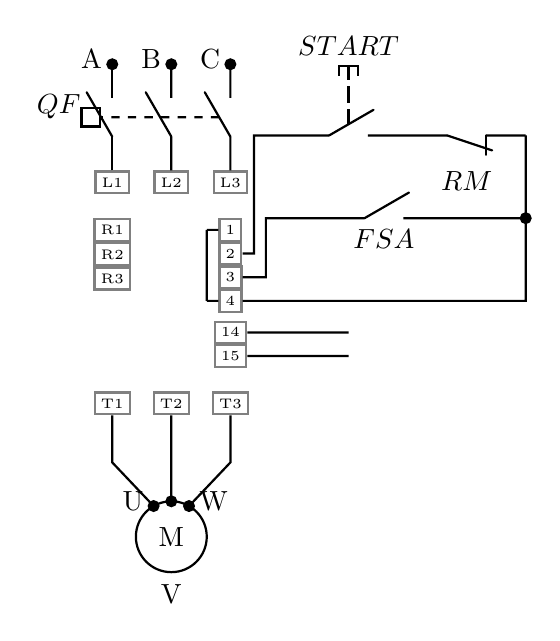
\begin{tikzpicture}[circuit ee IEC relay,thick,scale=1.5]
\draw (0.5,-0.7) ++(120:0.3)
node [contact,name=U,info={[left]:U}]{};
\draw (0.5,-0.7) ++(90:0.3)
node [contact,name=V,info={[below=1]:V}]{};
\draw (0.5,-0.7) ++(60:0.3)
node [contact,name=W,,info={[right]:W}]{};
\draw (0.5,-0.7) circle (0.3);
\node at(0.5,-0.7) {M};

\node[shape=rectangle,draw=gray,node font={\tiny}] (A1) at (0,2.3){L1};
\node[shape=rectangle,draw=gray,node font={\tiny}] (B1) at (0.5,2.3){L2};
\node[shape=rectangle,draw=gray,node font={\tiny}] (C1) at (1,2.3){L3};

\node[shape=rectangle,draw=gray,below=3mm of C1,node font={\tiny}] (a){1};
\node[shape=rectangle,draw=gray,below=0mm of a,node font={\tiny}] (b){2};
\node[shape=rectangle,draw=gray,below=0mm of b,node font={\tiny}] (c){3};
\node[shape=rectangle,draw=gray,below=0mm of c,node font={\tiny}] (d){4};

\node[shape=rectangle,draw=gray,below=1mm of d,node font={\tiny}] (e){14};
\node[shape=rectangle,draw=gray,below=0mm of e,node font={\tiny}] (f){15};

\node[shape=rectangle,draw=gray,below=3mm of A1,node font={\tiny}] (g){R1};
\node[shape=rectangle,draw=gray,below=0mm of g,node font={\tiny}] (h){R2};
\node[shape=rectangle,draw=gray,below=0mm of h,node font={\tiny}] (i){R3};

\node[shape=rectangle,draw=gray,below=25mm of A1,node font={\tiny}] (T1){T1};
\node[shape=rectangle,draw=gray,below=25mm of B1,node font={\tiny}] (T2){T2};
\node[shape=rectangle,draw=gray,below=25mm of C1,node font={\tiny}] (T3){T3};
to [make contact={term=1,term'=2}] ++(0,-1) -- (A1);
\draw (A1) to [make contact={name=QF3}] ++(0,1) node [contact,name=A,info={[left]:A}]{};
\draw (B1) to [make contact] ++(0,1) node [contact,name=B,info={[left]:B}]{};
\draw (C1) to [make contact={name=QF1}] ++(0,1) node [contact,name=C,info={[left]:C}]{};
\draw[dashed](QF1.mid) -- (QF3.mid)
node[left,draw,solid,minimum size=1mm,label={[left]:$QF$}]{};

\draw (T1) -- ++(0,-0.5) -- (U);
\draw (T2) --  (V);
\draw (T3) -- ++(0,-0.5) -- (W);

\draw (c) --  ++(0.3,0) -- ++(0,0.5)--++(0.5,0)
to [make contact={info={below:$FSA$}}] ++(1,0) -- ++(0.7,0)
node [contact,name=k]{};
\draw (b) -- ++(0.2,0) -- ++(0,1) -- ++(0.3,0)
to [make contact={push button={info=$START$}}] ++(1,0)
to [break contact={info={below:$RM$}}] ++(1,0)
node[shape=coordinate](k1){};
\draw (d) -- ++(2.5,0) -- (k1);
\draw (a) -- ++(-0.2,0) node[shape=coordinate](a1){};
\draw (d) -- ++(-0.2,0) node[shape=coordinate](d1){};
\draw (a1) -- (d1);
\draw (e) -- ++(1,0);
\draw (f) -- ++(1,0);
	\end{tikzpicture}
			\column{.4\textwidth}
\begin{block}{动力回路设备}
				\begin{enumerate}
				\item  空气开关(QF)
\begin{enumerate}
				\item  负荷6A
				\end{enumerate}
				\item  变频器(AB)
\begin{enumerate}
				\item  动作电流定值
				\item  复位方式(H/A)
				\end{enumerate}
				\item  变频电机(M)
\begin{enumerate}
				\item  散热
				\end{enumerate}

				\end{enumerate}
\end{block}
		\end{columns}
	\end{frame}
\begin{frame}{给煤机电气原理}{给煤机动力回路-变频器控制接线功能图}
  		\begin{columns}
			\column{.5\textwidth}
\begin{figure}
%\centering
%\includegraphics[angle=0,width=150pt,trim=10 50 0 80,clip]{1.pdf}
%\caption{两线制接线图}
	
\end{figure}
	\column{.5\textwidth}
\begin{block}{参数含义}
			\begin{enumerate}
				\item 标定过程中计量的物料量
				\item  修正系数KOR
				\end{enumerate}
\end{block}
\begin{exampleblock}{标定结果评估}
			\begin{description}
				\item[KOR=0.99...1.01]正常
				\item[KOR=0.95...1.05]修正P04.02
				\item[KOR=.0.95.1.05.]超出允许范围
				\end{description}
\end{exampleblock}
\begin{alertblock}{注意!!}
			
				手动修改P04.02
\end{alertblock}
		\end{columns}
	\end{frame}
\subsection{给煤机控制回路}
	\begin{frame}{给煤机电气原理}{给煤机控制回路}
		\begin{columns}
			\column{.7\textwidth}
		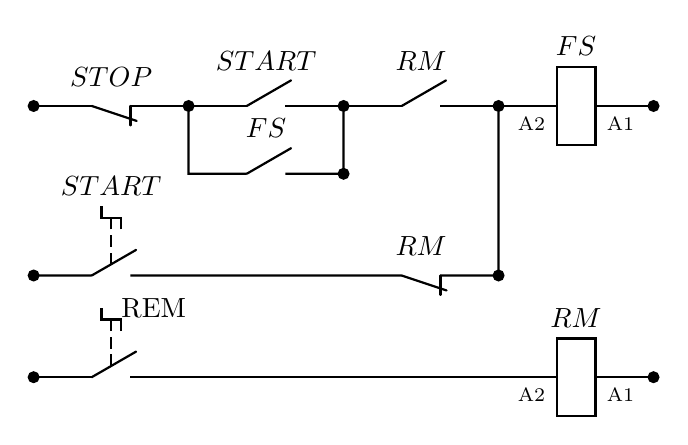
\begin{tikzpicture}[circuit ee IEC relay,thick,x=8\tikzcircuitssizeunit,y=3.5\tikzcircuitssizeunit]
		
		

		\draw (0,0)node [contact,name=A1]{}
		to [break contact={info=$STOP$}] ++(1,0)node [contact,name=A2]{}
		to [make contact={info=$START$}] ++(1,0)node [contact,name=A3]{}
to [make contact={info=$RM$}] ++(1,0)node [contact,name=A4]{}
		to [relay coil={info=$FS$,term=A1,term'=A2}] ++(1,0)node [contact,name=A5]{};
\draw (A2) -- ++(0,-1)
to [make contact={info=$FS$}] ++(1,0)node [contact,name=B1]{} --(A3);
	\draw (0,-2.5)node [contact,name=C1]{}
		to [make contact={turn switch={info=$START$}}] ++(1,0) -- ++(1,0)
		to [break contact={info=$RM$}] ++(1,0)node [contact,name=C3]{} -- (A4);

		\draw (0,-4)node [contact,name=D1]{}
		to [make contact={turn switch={info={[right]:REM}}}] ++(1,0) -- ++(2,0)
		to [relay coil={info=$RM$,term=A1,term'=A2}] ++(1,0)node [contact,name=D2]{};


	\end{tikzpicture}
			\column{.3\textwidth}
\begin{block}{控制回路设备}
				\begin{enumerate}
				\item  启动按钮START
\item  DCS启动脉冲
				\item  钮子开关GK
				\item  前进限位LSF
\item  后退限位LSR
\item  进接触器CFi
\item  退接触器CRi
\item  热继电器CRJi
				\end{enumerate}
\end{block}
		\end{columns}
	\end{frame}
\begin{frame}{参考文献}
\begin{thebibliography}{10}
	
\end{thebibliography}
\end{frame}
\end{document}
